\BourbakiExercisesSection

\begin{enumerate}
\def\labelenumi{\arabic{enumi}.}
\item
  给出交换环的一个同态 \(\rho: \mathbf{A} \to \mathbf{B}\) 以及两个 A-模 E、F 的例子，使得典范同态（17）（第 3 号）既不是单射也不是满射（参见 §4，习题 2）。
\item
  给出一个自由 A-模和一个环 B 的例子，使得同态（20）（第 4 号）不是单射（§3，习题 3）。
\item
  给出一个单生成 A-模 E 以及一个环 B 的例子，使得同态（20）（第 4 号）不是满射（参见 §4，习题 2）。
\item
  设 \(\rho: A \to B\) 是一个环同态。对于每个 A-模 \(E\) ，证明图表
\end{enumerate}

\pandocbounded{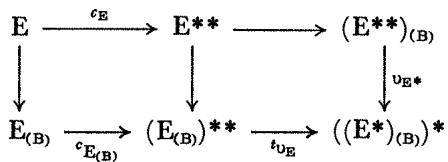
\includegraphics[keepaspectratio]{images/part003_7dd43288.jpg}}

是交换的。

\begin{enumerate}
\def\labelenumi{\arabic{enumi}.}
\setcounter{enumi}{4}
\item
  设 K 为一个域，A 为乘积环 \(K^{N}\) ，a 为 A 的理想 \(K^{(N)}\) ，B 为环 A/a。证明 a 是投射 A-模但不是有限生成的，尽管 \(a_{(B)} = \{0\}\) 。
\item
  设环 A 和 B 如 §1 习题 7 中所定义，令 M 为一个 A-模；证明 M 是有限生成的（相应地，自由的、投射的）当且仅当 \(M \otimes_{A} B\) 是有限生成的（相应地，自由的、投射的）。
\item
  设 \(\rho: A \to B\) 是一个环同态。对每个左 B-模 \(F\) ，定义典范的 B-模同态
\end{enumerate}

\[
\mathbf {F} \rightarrow \tilde {\rho} (\rho_ {*} (\mathbf {F}))
\]

并证明若 E 是一个左 A-模，则复合映射

\[
\begin{array}{r l} & {\tilde {\rho} (\mathbf {E}) \to \tilde {\rho} (\rho_ {*} (\tilde {\rho} (\mathbf {E}))) \to \tilde {\rho} (\mathbf {E})} \\ & {\rho_ {*} (\mathbf {F}) \to \rho_ {*} (\tilde {\rho} (\rho_ {*} (\mathbf {F}))) \to \rho_ {*} (\mathbf {F})} \end{array}
\]

是恒等映射。

